%% \listfiles
\documentclass[apj]{emulateapj}
%\documentclass[preprint2,12pt]{emulateapj}
%% \usepackage{natbib}
\usepackage{graphicx}
\usepackage{epsfig}
\usepackage{amssymb,amsmath}
\usepackage{array}
\usepackage{threeparttable}


\singlespace

%definitions
\newcommand{\Msol}{${\rm M_{\sun}}$}


%% Editing markup...
\usepackage{color}


%%%%%%%%%%%%%%%%%%%%%%%%%%%%%%%%%%%%%%%%%%%%%%%%%%%%%%%%%%%%%%%%%%%%%%%%%%%
% WARNING: This LaTeX block was generated automatically by authors.py
% Do not change by hand: your changes will be lost.

%%%%%%%%%%%%%%%%%%%%%%%%%%%%%%%%%%%%%%%%%%%%%%%%%%%%%%%%%%%%%%%%%%%%%%%%%%%


% --------------------- Ancillary information ---------------------
\shortauthors{SURP et al.}
\shorttitle{my short-title}
\slugcomment{\today}


\begin{document}

\title{A Graph Database Implementation for Astronomical Observatory
Hardware Tracking}
 %% ---------
 
\author{Zannatul S. Isaque\altaffilmark{1}, Supervisors: Prof. Adam Hincks, and Prof. Yilun Guan}
\altaffiltext{1}{CITA, University of Toronto}


 
\begin{abstract}
The Hydrogen Intensity and Real-time Analysis eXperiment (HIRAX) is an innovative observatory aiming to unravel the mysteries of the Universe by deploying a vast interferometric array of over 1,000 6 m radio dishes in the Karoo region of South Africa. Its primary objectives include studying the expansion history of the Universe and identifying and characterizing radio transients like pulsars and fast radio bursts. The successful implementation of HIRAX relies heavily on the development of an intricate data processing and reduction pipeline that necessitates meticulous coordination with the complex hardware layout. With each radio dish housing a dual polarisation antenna and a chain of cables, amplifiers, and filters leading to the digitiser, the task of tracing each digital signal back to its physical origin, precisely identifying the components it traverses, and accommodating the dynamic nature of the experiment pose significant challenges. As the experiment progresses, the number of components will rapidly increase, and adjustments will be made to ensure optimal performance. Meanwhile, the Simons Observatory, a next-generation ground-based telescope focused on measuring the Cosmic Microwave Background radiation, faces similar challenges in managing connected units and maintaining a timed record. To address these challenges, the versatile and improved design of padloper, a new system developed as an enhancement to the existing CHIME database, is poised to become an essential tool for data management in the Simons Observatory and other scientific experiments.
\end{abstract}

\keywords{telescopes, software, pulsars, cosmic microwave background radiation, cosmology, fast radio bursts}

\section{Introduction}
\label{sec:intro}
\begin{figure}
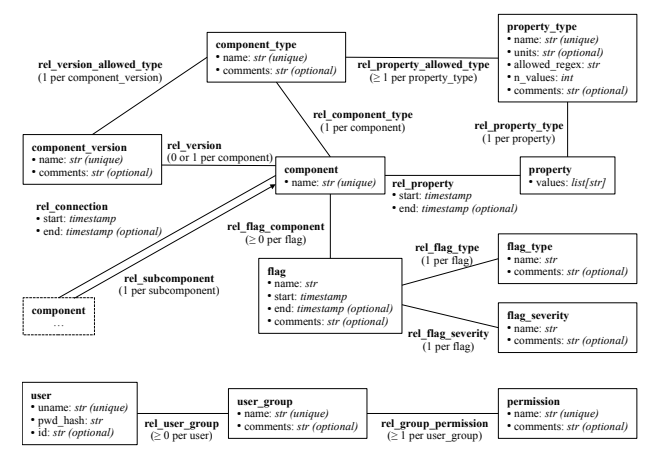
\includegraphics[width=1\columnwidth]{figs/save.png}
\caption{The database schema. Boxes are vertices, lines are edges, and text are vertex/edge
properties.\vspace{3mm}}
\label{fig:figureOfSpectrum}
\end{figure}

Padloper, a new system developed as an enhancement to the existing database system used by the Canadian Hydrogen Intensity Mapping Experiment (CHIME), aims to address the technical limitations and maintenance issues of its predecessor. With substantial contributions from previous SURP projects, padloper is being developed into a versatile tool that can be applied not only to HIRAX but also to other experiments such as those at the Simons Observatory. The Simons Observatory, a cutting-edge ground-based telescope focused on measuring the Cosmic Microwave Background radiation, presents similar challenges in managing a timed record of connected units, making padloper an essential tool for data management in a wide range of scientific endeavors. With its improved design and adaptability, padloper is poised to revolutionize the way data is handled and organized in the Simons Observatory and potentially numerous other scientific experiments.

\section{Janusgraph, Gremlin, and Padloper}
\label{sec:data}

I have successfully completed the installation of JanusGraph, a robust graph database system, and have gained proficiency in utilizing the Gremlin query language for database management. Moreover, I have installed gremlinpython and honed my skills in executing queries on the database using Python. Through hands-on exploration, I have actively experimented with different operations, enabling me to grasp the potential applications of this technology. To enhance my understanding, I have developed a concrete example that showcases the diverse functionalities and features offered by Gremlin. From my success with the installation of Janusgraph, Flask and React; I have gained some familiarity with padloper. However, there is still room for improvement in my understanding of utilizing the web interface effectively, as well as comprehending the dynamic relationship between the Flask and React servers and their integration with the Python API. Further investigation is necessary to deepen my comprehension of these components and their interactions.\\

\subsection{Data}
\label{sec:cmb_data}
Example, from HIRAX, of data we would come across during a telescope observation:
\begin{equation}  
\begin{bmatrix}
t & v & i & j\\
\end{bmatrix}
\label{eq:relativity}
\end{equation}
{Where t is time (10 seconds resolution), v is frequency, i and j are antenna polarisation}. The amount of data is in the billions, and this is why we need a bookkeeping software that tracks physical location, and configuration. (Hincks et al, 2022).

\section{Web Interface Frameworks}
\label{sec:data}
In my investigation of which Javascript Framework tool would be better at helping visualising graphs in the React web interface,  it is unfortunate to say that JSPlumb Community Edition was limited and faced some issues when it comes to seamless integration with React while maintaining a visually appealing interface. I have compared repositories of the two with JSPlumb and React Flow. Achieving a smooth and visually pleasing integration with JSPlumb becomes complex and error-prone. I would recommended continuing to use React Flow. However, an alternative library like React Dnd or Vue.js could be considered, as they are designed specifically for React and provide a more seamless integration for visually appealing interactions.

%\acknowledgments

\bibliographystyle{act}
 \bibliographystyle{apj}

\bibliography{lenscib_refs.bib,apj-jour}
Hincks, A. D., Zavyalov, A., and Bansal, D., “A graph database solution for tracking the deployment and layout of a large radio interferometer”, in <i>Society of Photo-Optical Instrumentation Engineers (SPIE) Conference Series</i>, 2022, vol. 12189. doi:10.1117/12.2627960.


\end{document}